\documentclass[12pt,letterpaper]{report}
\usepackage[utf8]{inputenc}
\usepackage[spanish]{babel}
\usepackage{amsmath}
\usepackage{amsfonts}
\usepackage{amssymb}
\usepackage{amsbsy}
\usepackage{graphicx}
\usepackage[left=3cm,right=2.5cm,top=3cm,bottom=2cm]{geometry}
\author{Fernando Manzanares}
\title{Seminario II}
\setlength{\parskip}{4mm}
\usepackage{ragged2e}
\justifying
\usepackage{longtable}
\usepackage{Sweave}
\setlength\parindent{1.25cm}
\usepackage{setspace}
\usepackage{titlesec} 
\usepackage{xcolor}
\titleformat{\chapter}[display]{\bfseries\Huge}{Capítulo \ \Huge\thechapter.}{0.5em}{}
\titlespacing{\chapter}{0pt}{0ex}{1pc}
\usepackage{upgreek}
\widowpenalty=10000  
\clubpenalty=10000
\usepackage{multirow}
\setcounter{secnumdepth}{3} 
\setcounter{tocdepth}{4} 
\usepackage{fancyhdr}
\renewcommand{\labelitemi}{•}
\usepackage{apalike}
\usepackage{cite}
\usepackage{subfigure}
\usepackage{caption}
\captionsetup [table]{name=Tabla}
\captionsetup [figure]{name=Gráfico}


\begin{document}
\Sconcordance{concordance:T_D_SII.tex:T_D_SII.Rnw:%
1 34 1}
\Sconcordance{concordance:T_D_SII.tex:./Portada.Rnw:ofs 35:%
1 28 1}
\Sconcordance{concordance:T_D_SII.tex:T_D_SII.Rnw:ofs 64:%
37}
\Sconcordance{concordance:T_D_SII.tex:./Indice.Rnw:ofs 65:%
1 2 1}
\Sconcordance{concordance:T_D_SII.tex:T_D_SII.Rnw:ofs 68:%
39}
\Sconcordance{concordance:T_D_SII.tex:./Abstract.Rnw:ofs 69:%
1 3 1}
\Sconcordance{concordance:T_D_SII.tex:./Introduccion.Rnw:ofs 73:%
1 20 1}
\Sconcordance{concordance:T_D_SII.tex:./PdelPro.Rnw:ofs 94:%
1 20 1}
\Sconcordance{concordance:T_D_SII.tex:./AbordajeT.Rnw:ofs 115:%
1 3 1}
\Sconcordance{concordance:T_D_SII.tex:T_D_SII.Rnw:ofs 119:%
44 5 1}


\spacing{1.5}

\thispagestyle{empty}

\begin{center}
UNIVERSIDAD DE EL SALVADOR \\ FACULTAD MULTIDISCIPLINARIA DE OCCIDENTE \\ DEPARTAMENTO DE MATEMÁTICAS \\
LICENCIATURA EN ESTADÍSTICA\\
\bigskip

\includegraphics [width=5cm,height=6cm]{Minerva}
\bigskip
\\ ANALISIS DE LA EFICIENCIA ENERGETICA EN LA UNIVERSIDAD DE EL SALVADOR FACULTAD MULTIDISCIPLINARIA DE OCCIDENTE \\
\bigskip
\textbf{MATERIA:}\\ 
SEMINARIO II\\
\textbf{ALUMNO:}\\ 
FERNANDO ERNESTO MANZANARES MORÁN\\
\bigskip
\bigskip
\bigskip
\bigskip
\bigskip
\bigskip

\textbf{SANTA ANA,    DICIEMBRE 2015,   EL SALVADOR}\\
\textbf{CENTRO AMÉRICA}\\


\end{center}


\spacing{1.0}

\tableofcontents 
\thispagestyle{empty}
\spacing{1.5}
\chapter*{Abstract}
\addcontentsline{toc}{chapter}{Abstract}
\pagenumbering{arabic}
Erase una vez...
\chapter*{Introducción}
\addcontentsline{toc}{chapter}{Introducción}

En la actualidad el medio ambiente es uno de los factores más tomados en cuenta con respecto
a la eficiente utilización de los recursos que éste entrega, además de la utilización de técnicas
estadísticas que aporten información para la correcta interpretación de la eficiencia con la que
dichos recursos son utilizados, estas son unas de las razones por la que investigaciones como esta
son necesarios para alcanzar la contribución efectiva en la protección del ambiente, en
términos generales, esta investigacion tiene como objetivo la provisión de 
un diseño favorable en cuanto analsis estadistico, sustentabilidad
ambiental, para alcanzar la eficiencia energética,
normalmente, los aspectos energéticos en cuanto a eficiencia están asociados a la especificación de
las potencias o capacidades de los equipos utilizados en la localización física y geográfica
donde se se encuentran ubicados, y su objetivo principal es alcanzar la utilización máxima de la
capacidad de los aparatos eléctricos con el menor consumo de energía posible, es decir a
través de actividades y tareas como el mantenimiento de sistemas y aparatos eléctricos, por esa
razón se busca la creación de una propuesta para alcanzar dicha eficiencia con el
fin de crear conciencia ambiental en las personas en general, en la UES FMOcc y lograr la
contribución al ambiente a través del ahorro de energía, además de sentar un precedente para
el análisis de datos, que se realizara a través de una serie de tiempo con el objetivo de alcanzar
el preciso análisis de los datos y así tomar la decisiones que generen mayor impacto ambiental.
\chapter{El Problema}
\section{Planteamiento del problema}
Desde hace ya varios años, la protección al medio ambiente se ha ido convirtiendo en un tema de mucha importancia,
tanto así, que varios países del mundo han comenzado a adoptar políticas para la conservación de este, dichas politicas van desde, el tratamiento desechos solidos hasta el ahorro de energía y cada día que pasa se adoptan muchas mas; entonces la NO protección del ambiente esta generando dichas reacciones en las poblaciones de todos los países alrededor del mundo, ya que en la actualidad se viven problemas como la contaminación y escasez de agua, contaminación del aire, degradación de los suelos y descenso de la productividad agrícola, deforestación, residuos sólidos y peligrosos, pérdida de la diversidad biológica, desgaste de la capa de ozono y cambios climáticos,todos estos problemas afectan a los países, de manera desigual, según el grado de su desarrollo, de su estructura económica y de las políticas ambientales que aplican, es decir para combatir el deterioro ambiental se llevan a cabo dos tipos de políticas; las que procuran relacionar el desarrollo con el medio ambiente a nivel general de población, recursos, legislación y tecnologías, y las que se orientan a problemas específicos, uno de los factores mas importantes al interior de estas problemáticas es el ahorro de energía, este factor entra en el segundo tipo de política anteriormente mencionada, es por eso que paises desarrollados están comenzando a implementar medidas que buscan dicho ahorro y ademas buscan consumir energía pero de manera eficiente.

En El Salvador, el problema de la eficiencia enérgetica no ha sido abordado desde el punto de vista estadistico, es decir, la aplicación de tecnicas estadisticas para investigar dicho problema,
normalmente, los aspectos energéticos en cuanto a eficiencia están asociados a la especificación de
las potencias o capacidades de los equipos utilizados en la localización física y geográfica
donde se se encuentran ubicados, y su objetivo principal es alcanzar la utilización máxima de la
capacidad de los aparatos eléctricos con el menor consumo de energía posible, por esa razon esta investigación busca la implementación de una serie temporal para el analisis de los datos del consumo electrico mensual en la Universidad de El Salvador Facultad Multidisciplinaria de Occidente (UES FMOcc), además, desarrollar proyeciones apartir de dicho modelo para analizar e interpretar el comportamiento del consumo eléctrico y sentar un presedente a nivel academico y teórico sobre el abordaje que se le pueden dar a este tipo de problemas, a estose agrega, contribuir en la protección del ambiente y generar conciencia para cambiar los habitos del consumo electrico, en la misma linea tambien pretende responder a las siguientes preguntas ¿Será eficiente el consumo eléctrico en la UES FMOcc? ¿Es posible alcanzar la eficiencia enérgetica en los edificios y aulas de la UES FMOcc? ¿Está el consumo energetico en la UES FMOcc creciendo a través del tiempo? ¿Cuáles son los periodos de tiempo donde se consume mas energia eléctrica? ¿Cuánta energía podria ahorrase si se lograra la eficiencia enérgetica?

\newpage
\section{Justificación}
Esta investigación pretende analizar y desarrollar proyeciones sobre los datos del consumo electrico en la UES FMOcc, para descubrir si existe o no eficiencia energetica además de la aplicación de un modelo estadistico autoregresivo integrado de media movil para datos estacionales y de esta manera poder interpretar los datos del consumo energetico de manera nueva y mas precisa, la importancia de realizar esta investigación se basa principlamente en el aporte teórico nuevo que sentara una base para el desarrollo de futuras investigaciones de esta índole, además de la aplicacion de tecnicas propiamente estadisticas para el monitoreo del comportamiento del consumo enérgetico en la UES FMOcc, esto con el fin de identificar los espacios de de tiempo donde se consume la mayor cantidad de energía eléctrica y de esta manera poder abordar de manera efectiva la problemática de eficiencia enérgetica, a esto se agrega que esta investigación tracenderá en el tiempo y será util durante los proximos 18 meses apartir de agosto de 2015 debido al tipo de tecnica utilizada para desarrollar las proyeciones y por último la contribución a la protección del ambiente una vez alcanzada la eficiencia en los sistemas electricos de la UES FMOcc, en el aspecto económico la realización de esta investigación resultaria favorable ya que la eficiencia enérgetica ademas de contribuir al ambiente sugiere una reducción en los costos del consumo enérgetico. 


\newpage
\section{Objetivos de la investigación}
\subsection{Objetivo general}

\begin{itemize}
\item Analizar los datos del consumo eléctrico a través de la utilización de una serie
temporal, para la interpretación de el comportamiento del consumo enérgetico a través del tiempo y si existe eficiencia energética en la UES FMOcc en los próximos 18 meses.
\end{itemize}

\subsection{Objetivos específicos}

\begin{itemize}
\item Desarrollar y analizar las proyecciones de los datos del consumo eléctrico de la
FMOcc a través de modelos estadísticos de series temporales para los próximos 18
meses.

\item Identificar el periodo de tiempo donde el consumo energetico es mas bajo y analogamente donde es mas alto.

\item Conecer la cantidad de energia y costos que podrían reducirse para contribuir al ambiente si se lograra la eficiencia energetica.  

\end{itemize}

\newpage
\section{Hipótesis}
\textbf{ Hipotesis 1.} 

$H_0$ No existe eficiencia energetica en los edificios de la Universidad de El Salvador Facultad Multidisciplinaria de Occidente.

$H_1$ Existe eficiencia energetica en los edificios de la Universidad de El Salvador Facultad Multidisciplinaria de Occidente.

\textbf{ Hipotesis 2.}

$H_0$ El consumo energetico en la Universidad de El Salvador Facultad Multidisciplinaria de Occidente es creciente a través del tiempo.

$H_1$ El consumo energetico en la Universidad de El Salvador Facultad Multidisciplinaria de Occidente no es creciente a través del tiempo.


\textbf{ Hipotesis 3.}

$H_0$ Los periodos donde más energia electrica se consume son durante los ciclos academicos desarrollados en la Universidad de El Salvador Facultad Multidisciplinaria de Occidente. 

$H_1$ Los periodos donde más energia electrica se consume no son durante los ciclos academicos desarrollados en la Universidad de El Salvador Facultad Multidisciplinaria de Occidente.





\chapter{Fundamentación teórica}
\section{Antecedentes}
  \subsection{Eficiencia Energetica en España}

    La eficiencia enérgetica 



\section{Teorías acerca de la eficiencia enérgetica}

\section{Teorías estadísticas}

  \subsection{Estacionariedad, Estacionalidad y transformaciones}

Los datos en los negocios, ingeniería, medicina y en otras áreas de investigación científica generalmente se recolectan en forma de series temporales, es decir, son recolectados de manera secuencial en un lapso determinado de tiempo que generalmente describen el comportamiento de una o varias variables que son observadas, de manera específica el objetivo principal que persigue una serie temporal es: entender e interpretar la dinámica de estructuras dependientes que forman las observaciones en el tiempo consigo mismas (de una variable, que se retroalimenta) o el efecto que pueden tener las relaciones de este tipo de estructuras temporales con otras (varias variables); los beneficios que puede lograr el claro entendimiento de este tipo de estructuras temporales son principalmente las predicciones precisas de las observaciones en el futuro en una variedad de esquemas de información en este caso el del consumo energético.

"Formalmente una serie de tiempo se define como un conjunto de observaciones repetidas de la misma variable tal como:$ Y_1, Y_2, · · · , Y_T$. A partir de esta caracterización se desprenden dos conceptos fundamentales en el análisis de series de tiempo. Los mismos se definen mediante la imposición de algunos supuestos
sobre el comportamiento de $Y_t$". \cite{Isaac}

Uno de estos supuestos es la estacionariedad de una variable observada en el tiempo ($Y_t$); de manera teórica, esto equivale a decir que las observaciones están fluctuando en torno a un mismo valor, es decir dichas observaciones poseen media constante, además para complementar este concepto es necesario tomar en cuenta que los datos observados deben estar fluctuando de manera similar en un lapso de tiempo, en otras palabras deben poseer varianza constante, a esto se agrega que la covarianza entre dos observaciones dependa únicamente de su separación y no del instante en el tiempo en el que se toman, en la misma línea cabe destacar que en la práctica, la mayoría de las series que se analizan poseen ausencia de estacionariedad, es decir, no poseen media ni varianza constante y que la covarianza depende del instante del tiempo y no de su separación  (son no estacionarias), de manera formal es posible definir que para el análisis de una serie temporal, la estacionariedad, es estrictamente necesaria, ya que si una serie cumple esta condición esta será invariante en el tiempo (en teoría), esta es una de las condiciones más fuertes que debe cumplir una serie en el tiempo.

El autor \cite{Tsay}, define de manera formal la estacionariedad (debil) de una serie de tiempo si se cumple:

\begin{enumerate}
\item $E(Y_t) = \mu$
\item $Cov(Y_t,Y_{t-\ell}) = Y_\ell$, y solo depende de $\ell$.
\end{enumerate}

Otro concepto importante es el de la estacionalidad, esto quiere decir que la serie temporal presenta un comportamiento cíclico, es decir dicho ciclo puede repetirse semanal,  mensual, trimestral, semestral e incluso anualmente, todo depende del tipo de variable que se esté observando, cuando esta característica está presente la serie adopta el nombre de serie de tiempo estacional, para el análisis de este tipo de series es necesario aplicar ciertos procedimientos para lograr un ajuste estacional (remover la estacionalidad) y luego conseguir que esta nueva serie cumpla la condición de ser estacionaria; para saber si una serie es estacional, se utiliza el correlograma comúnmente denominado grafico de auto correlaciones simples, donde se observan los retardos con mayor correlación durante un lapso determinado de tiempo esto con el fin de encontrar cierta repetitividad en cada periodo observado, posteriormente una vez detectada la estacionalidad pueden utilizarse técnicas como la diferenciación estacional definida por, $\triangle_s Y_t = y_{t}-y_{t-s}$; de una serie estacional $Y_t$ con periodicidad "s", cabe mencionar que esta expresión es similar a la diferenciación para una serie no estacional $Y_t$, definida por $Y_t=y_{t}-y_{t-1}$; \cite{Tsay}

Una vez detectada la estacionalidad o la no estacionalidad de la serie, es necesario que la serie sea estacionaria, para lograr esto, se utiliza comúnmente la técnica de diferenciación no estacional y la diferenciación estacional, esta última solo si la serie es estacional, este proceso se lleva a cabo para lograr que la serie sea constante en media; para conseguir varianza constante comúnmente se utilizan transformaciones de escala como la logarítmica o se usa la transformacion de box-cox para tomar la mejor decisión, dicha transformacion esta definida por:

\begin{center}
$f(x) = \left\{
\begin{matrix}
  \dfrac{x^\lambda - 1}{\lambda}   &  \mbox{para } \lambda \not= 0 \\
    log(x)                        &   \mbox{para } \lambda = 0 
\end{matrix}\right.$
\end{center}

Esta transformación consiste en calcular un valor de lambda y aplicar la transformación, cabe mencionar que si $\lambda$ se aproxima a cero la transformacion equivale a el $log(x)$ si $\lambda$ es igaual a $\frac{1}{2}$ la tranasformación equivale a la raiz cuadrada y si $\lambda$ es igual a $-1$ enconces multiplicar por el reciproco de cada dato sería su equivalente, algunos programas estadísticos facilitan el calculo de $\lambda$ a partir de los datos en esta investigación se utilizara el programa R.\cite{Cryer}

Ahora necesario probar estadisticamente si la serie es estacionaria, para eso se utiliza la prueba de Dickey Fuller (DF) que contrasta la hipótesis nula de que una serie es no estacionaria si el polinomio asociado a esta posee raíz unitaria, la decisión sobre este contraste se toma a partir del valor asintótico (P-valor) arrojado por la prueba, si este es menor a la significancia utilizada entonces se rechaza la hipótesis nula y puede concluirse que la serie es estacionaria, por último es importante mencionar que “el test DF, es poco potente, corremos por tanto el riesgo de admitir la presencia de una raíz unitaria cuando en realidad no existe” \cite{Ramon}. En la misma línea debe saberse por que tomar la decisión de utilizar una prueba como la de DF para probar estacionariedad, se sabe que una variable simple auto regresiva tiene la forma $x_t=\alpha x_{t-1}+\varepsilon_t$; \cite{Daniel2001}, si se sustrae $x_{t-1}$ de ambos lados el resultado es $\triangle x_t=(\alpha-1) x_{t-1}+\varepsilon_t$; esta ecuación es la base de la prueba DF, “el estadístico de prueba es el estadístico t sobre la variable rezagada. Si $\alpha>1$ el coeficiente de la variable rezagada será positivo, si "$\alpha$" es igual a la unidad $(\alpha-1)$ será igual a cero. En ambos casos $x_t$ será no estacionaria” \cite{Commandeur2007}.

\subsection{Función de autocorrelacion simple (FAS o ACF)}

Cuando se mide una variable a lo largo del tiempo, las observaciones en
diferentes periodos a menudo están relacionadas o correlacionadas. Esta correlación se mide usando el coeficiente de autocorrelación. La autocorrelación
es la correlación que existe entre una variable retrasada uno o más períodos
consigo misma.
Los patrones de datos que incluyen componentes como tendencia y estacionalidad pueden estudiarse usando autocorrelaciones. Los patrones se identifican
examinando los coeficientes de autocorrelación de una variable en diferentes
retrasos de tiempo.

La ecuación siguiente ecuacion es la fórmula para calcular el coeficiente de autocorrelación $r_k$
entre las observaciones $Y_t$ y $Y_{t-k}$, que se encuentran a k periodos de distancia.

\begin{center}
$\rho_k = \dfrac 
{\sum_{t=k+1}^{n} (Y_t-\bar{Y})(Y_{t-k}-\bar{Y})}
{\sum_{t=1}^{n} (Y_t - \bar{Y})^2}; \mbox{ Para } k = 1,2,3,...$
\end{center}

Donde,

\textbf{$\rho_k$}: Es el coeficiente de autocorrelación para un retraso de k periodos.

\textbf{$\bar{Y}$}:Es la media de los valores de la serie de tiempo.

\textbf{$Y_t$}:Es la observación en el periodo t.

\textbf{$Y_{t-k}$}:  Es la observación k periodos anteriores o durante un periodo t - k.

\subsection{Función de autocorrelacion parcial (FAP o PACF)}

La autocorrelacióon parcial mide la correlación entre dos variables separadas por k periodos cuando no se considera la dependencia creada por los retardos intermedios existentes entre ambas, Los coeficientes de autocorrelaci´on para diferentes retrasos de tiempo de una
variable pueden usarse para contestar las siguientes preguntas acerca de una
serie de tiempo:

\begin{enumerate}
\item  Los datos son ruido blanco.\footnote{El proceso t se define como ruido blanco si cumple con
las siguientes condiciones:\\
1. La esperanza de $Y_t$ o promedio es igual a 0 para todos los periodos t. Esto es $E(Y_t) = 0$ para toda t.\\
2. La varianza de $Y_t$ es constante y por consiguiente independiente del tiempo. Esto es $var(Y_t) = \sigma^2$.}
\item  Los datos muestran una tendencia (son no estacionarios).
\item  Los datos son estacionarios.
\item  Los datos son estacionales.
\end{enumerate}

Si una serie es aleatoria, las autocorrelaciones entre $Y_t$ y $Y_{t-k}$ para cualquier
retraso de tiempo k son cercanas a cero. Los valores sucesivos de una serie
de tiempo no est´an relacionados entre sí. "Si una serie muestra una tendencia,
las observaciones sucesivas están altamente correlacionadas y es típico que
los coeficientes de correlación sean significativamente diferentes de cero, para
los primeros retrasos de tiempo, y de forma gradual tienden a cero conforme
se incrementa el número de retrasos" \cite{Isaac}.

Para identificar si una autocorrelacion es significativamente diferente de cero se utiliza el correlograma, y apartir de este se toma la decisión sobre los retardos, por ejemplo:

\begin{figure}[htb]

\centering
\caption{Correlograma} 
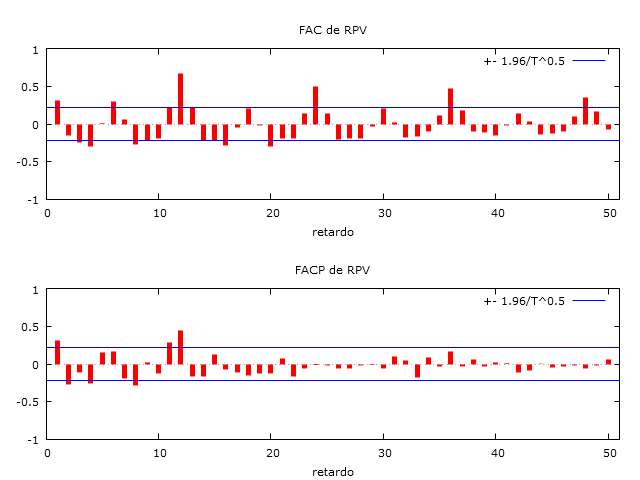
\includegraphics [width=0.8\textwidth]{LOL2}
\label{correlograma1}
\end{figure}

De este correlograma puede observarse que las barritas son la representacion de la correlacion de los retardos y las que no se salen de las lineas horizontales son significativamente iguales a cero y las que no se salen son los retardos con correlacion significativamente diferente de cero.

\textbf{¿Cómo identificar cuando los datos de una serie muestran tendencia?}

Si una serie muestra una tendencia, hay una relación significativa entre los
valores sucesivos de la serie de tiempo. Los coeficientes de autocorrelación son
usualmente grandes para varios de los primeros retrasos de tiempo y luego,
conforme se incrementa el número de retrasos, caen gradualmente hacia cero; 
Una serie de tiempo estacionaria es aquella cuyas propiedades estadísticas
básicas, como la media y la varianza, permanecen constantes en el tiempo,
por lo tanto, se dice que una serie que varía alrededor de un nivel fijo (sin
crecimiento ni decrecimiento) con el paso del tiempo es estacionaria, se dice
también que una serie que contiene una tendencia es no estacionaria, los
coeficientes de autocorrelación de una serie estacionaria decrecen hacia cero
bastante rápidamente, por lo común después del segundo o tercer retraso
de tiempo, por otro lado, las autocorrelaciones muestrales de serie no estacionaria se permanecen muy grandes durante varios periodos.

\textbf{¿Cómo identificar estacionalidad en una serie temporal?}

Si una serie es estacional, un patrón relacionado con el calendario se repite
así mismo durante un intervalo de tiempo específico (generalmente un año).
Las observaciones de la misma posición, en diferentes periodos estacionales,
tienden a estar relacionadas. Si se analizan datos trimestrales que tienen un
patrón estacional, los primeros trimestres tienden a parecerse, los segundos
trimestres tienden a parecerse, y así sucesivamente, y habrá un coeficiente de
autocorrelación significativo en el retraso de tiempo 4, si se analizan datos
mensuales, aparecer´a un coeficiente de autocorrelación significativo en el retraso de tiempo 12, es decir, enero se correlacionará con otros eneros, febrero
se correlacionará con otros febreros y así sucesivamente, un ejemplo de ello se nota en el gráfico \ref{correlograma1} para un retraso de tiempo 12.

\subsection{Metodología Box-Jenkins}

La metodología Box-Jenkins para generar pronósticos es diferente de la
mayoría de los métodos porque no supone ningún patrón particular en los
datos históricos de las series que se van a pronosticar, se basa en un enfoque iterativo para identificar un modelo posible a partir de una clase general
de modelos, luego, el modelo seleccionado se coteja con los datos históricos
para ver si describe la serie con exactitud, el modelo está bien ajustado si
los residuos son generalmente pequeños, están distribuidos aleatoriamente y
no contienen información útil, si el modelo especificado no es satisfactorio,
el proceso se repite usando un nuevo modelo diseñado para mejorar el original, este procedimiento iterativo continúa hasta que se encuentra un modelo
satisfactorio, en ese momento, el modelo se considera útil para pronosticar.
La selección inicial de un modelo ARIMA se basa en examinar una gráfica
de la serie de tiempo (para observar su carácter general) y en analizar sus
autocorrelaciones para varios retrasos de tiempo, específicamente, el patrón
de las autocorrelaciones muestrales calculado a partir de la serie de tiempo
se coteja con el patrón conocido de autocorrelación asociado con un modelo
ARIMA particular, este acoplamiento se hace tanto para las autocorrelaciones como para las autocorrelaciones parciales \cite{Isaac}.

\subsection{Modelo autoregresivos integrados de media movil ARIMA(p,d,q)}

Este modelo es la composicion de un modelo AR(p) y un MA(q) \cite{Cryer} y tambien esta basado en el
supuesto de estacionariedad, esto es, la media y la varianza para una serie de
tiempo son constantes en el tiempo y la covarianza es invariante en el tiempo,
pero se sabe que muchas series de tiempo y en especial las series económicas
no son estacionarias, porque pueden ir cambiando de nivel en el tiempo o
sencillamente la varianza no es constante en el tiempo, a este tipo de proceso
se les considera procesos integrados, por consiguiente, se debe diferenciar
una serie de tiempo "d" veces para hacerla estacionaria y luego aplicarla a esta
serie diferenciada un modelo ARMA(p, q) , se dice que la serie original es
ARIMA(p, d, q)\footnote{Observe que cuando q = 0, el modelo ARMA(p, 0) se reduce a un modelo autorregresivo puro de orden p, de forma similar, cuando p = 0, el modelo ARMA(0, q) es un
modelo de promedio móvil puro de orden q}, es decir, una serie de tiempo autoregresiva integrada de
media m´ovil, donde "p" denota el número de términos autoregresivos, "d" es el
número de veces que la serie debe ser diferenciada para hacerla estacionaria
y "q" el número de términos de la media móvil.

El modelo teórico es el siguiente:

$(1-\phi_1 B - \phi_2 B^2 - ... - \phi_p B^p)(1-B)^d Y_t = (1-  \theta_1 B- \theta_2 B^2-· · ·- \theta_q B^q)\varepsilon_t$

$B^k(Y_t) = Y_{t-k}$ es el operador de retardos o retroactivo.

\subsection{Proceso estacional autoregresivos integrados de media movil SARISMA(P,D,Q)}

Segun \cite{Cryer} cuando una serie de tiempo en estudio tiene intervalos de observación menores a un año, entonces es frecuente que estas tengan variaciones o patrones
sistemáticos cada cierto periodo, estas variaciones sistemáticas inferiores a un
año por ejemplo semestral, mensual, diario, etc., deben ser captadas en los
llamados "Factores Estacionales", dentro de la estructura del modelo a construirse, cada una de estas series puede ser estacionaria o no estacionaria, de
esta manera se combinan términos ordinarios del proceso ARMA y términos
estacionales, así como diferencias regulares y diferencias estacionales para
transformar en series estacionarias; este tipo de procesos
tiene las siguientes características:

\begin{enumerate}

\item Contiene una componente ARIMA(p, d, q) que modela la dependencia regular, que es la dependencia asociada a observaciones consecutivas.

\item Contiene una componente ARIMA(P, D, Q) que modela la dependencia estacional, que está asociada a observaciones separadas por periodos.

\end{enumerate}

El modelo teórico es el siguiente:


$Y_t = c + \overbrace{\phi_1 Y_{t-1}+ ... + \phi_p Y_{t-p}}^{AR(p)}+ \overbrace{\Phi_1 Y_{t-s}+\Phi_2 Y_{t-2s}+...+\Phi_p Y_{t-P_s}}^{SAR(P)} + \\ \underbrace{\varepsilon_t - \theta_1 \varepsilon_{t-1} -...- \theta_q \varepsilon_{t-q}}_{MA(q)} - \underbrace{\Theta_1 \varepsilon_{t-s} - ... - \Theta_q\varepsilon_{t-Q_s}}_{SMA(Q)}$



\subsection{Seleccion, validación del modelo y elaboracion de pronósticos}

\textbf{Selección del modelo}

Para tener una idea del valor de p,q,P y Q para el modelo ARIMA(p,d,q)*(P,D,Q) se hacen uso de las herramietas graficas: Correlogramas, Correlograma extendido, una vez selecionado los valores de p,q,P y Q, se prueban los modelos y se comparan con los criterios de selecion AIC, BIC \cite{Shumway}, cuando ya se ha selecionado el modelo con el menor valor de AIC y BIC entonces se procede a la validación.

\textbf{Validación del modelo}

Para validar el modelo selecionado deben de cumplirse los siguientes supuestos:

\begin{enumerate}
 \item Debe probarse que los residuos del modelo tienen una distribución normal. 
 \item Los resíduos deben tener media 0 y varianza constante (ser ruido blanco).
 \item Las autocorrelaciones residuales individuales deben ser pequeñas y generalmente dentro de         la banda del correlograma y deben ser muy próximas a cero.
 \item Las autocorrelaciones residuales como un grupo deben ser congruentes con aquellas producidas por los errores aleatorios, una verificación
general de la idoneidad del modelo se realiza mediante una prueba de
distribución chi cuadrada $(\emph{X}^2)$ con base en el estadísstico Q de LjungBox\footnote{Si el valor p asociado con el estadístico Q es pequeño (digamos, el valor
p < 0,05), el modelo se considera inadecuado.}

\end{enumerate}

\textbf{Elaboración de pronósticos}

Una vez que se ha encontrado un modelo adecuado, es factible elaborar los pronósticos de uno o varios periodos futuros, con base en los
pronósticos también se pueden construir intervalos de predicción, en
general, para un nivel de confianza dado, cuanto más largo sea el tiempo guía del pronóstico, mayor será el intervalo de predicción, esto es
razonable, puesto que se espera que la incertidumbre sea mayor para
el pronóstico de un valor distante que para el pronóstico de, digamos,
la siguiente observación. El cálculo de los pronósticos e intervalos de
predicción es una labor tediosa y es preferible dejarla a la computadora,
los programas de computadora que ajustan modelos ARIMA generan
pronósticos e intervalos de predicción a requerimiento del analista \cite{Isaac}.






\nocite{*}
\bibliographystyle{apalike}
\bibliography{SIIB}

\end{document}





